%%%%%%%%%%%%%%%%%%%%%%%%%%%%%%%%%%%%%%%%%%%%%%%%%%%%%%%%%%%%%%%%%%%%%%%%%%%%%%%%
%                     Bachelor thesis template
%						 Science Faculty
%								at
%			National Autonomous University of Mexico (UNAM)
%%%%%%%%%%%%%%%%%%%%%%%%%%%%%%%%%%%%%%%%%%%%%%%%%%%%%%%%%%%%%%%%%%%%%%%%%%%%%%%%
% based on Harish Bhanderi's PhD/MPhil template, then Uni Cambridge
% http://www-h.eng.cam.ac.uk/help/tpl/textprocessing/ThesisStyle/
% corrected and extended in 2007 by Jakob Suckale, then MPI-iCBG PhD programme
% and made available through OpenWetWare.org - the free biology wiki
%
%                     Under GNU License v3
%
% Adapted for the Engineering School at UNAM by Jesús Velázquez y Marco Ruiz
% Then, adapter fot he Science Faculty at UNAM by Jonathan Urrutia
%
%
%
% All used packages are found in
%
%					./Latex/Classes/PhDthesisPSnPDF.cls
%
% within this las documments there are some lines to be UnCommented for a printed or a digital version of the output file:
%
%			line 184
%			lines 231-261
%
%	Since this is a template for a thesis made at UNAM (Mexico) the titles may be in spaninish but within PhDthesisPSnPDF.cls it can be change
%

\documentclass[11pt]{Latex/Classes/PhDthesisPSnPDF}

\usepackage{blindtext}         %  For dummy text.
% The \blindtext or \Blindtext commands throughout this template generate dummy text to fill the template out.

\include{Latex/Comands}           % Special commands written by the author

\usepackage{setspace}
\usepackage{layouts}
\svgpath{{1-Theory-Figs}}

\usepackage{lmodern}

\usepackage{Latex/mmacells}


\mmaDefineMathReplacement[≤]{<=}{\leq}
\mmaDefineMathReplacement[≥]{>=}{\geq}
\mmaDefineMathReplacement[≠]{!=}{\neq}
\mmaDefineMathReplacement[→]{->}{\to}[2]
\mmaDefineMathReplacement[⧴]{:>}{:\hspace{-.2em}\to}[2]
\mmaDefineMathReplacement{∉}{\notin}
\mmaDefineMathReplacement{∞}{\infty}
\mmaDefineMathReplacement{𝕕}{\mathbbm{d}}


\mmaSet{
  morefv={gobble=2},
  linklocaluri=mma/symbol/definition:#1,
  morecellgraphics={yoffset=1.9ex}
}
%%-------------------------------------------------------------------------------
%                                  Information of the Student
%-------------------------------------------------------------------------------
% --- Default information for Bachelor's degree
%\author{Jonathan Alexis Urrutia Anguiano}
%\title{Optical response of partially embedded nanospheres}
%\programa{Posgrado en Ciencias Físicas} % Licenciatura en Física
%\degree{Maestro en Ciencias}% Maestro en / Doctor en
%\director{Dr. Alejandro Reyes Coronado}% Thesis director
%\facultad{Facultad de Ciencias}
%\lugar{Ciudad de México, México}% Place of the dissertation
%\degreedate{2021}% Year of the dissertation
%\portadatrue   %Uncomment for color cover

% ----------------------------- Datos del jurado de Licenciatura
%\student{Paternal last name\\ Maternal Last name\\ Names\\ Telephone number\\ Universidad Nacional Autónoma de México\\ Facultad de Ciencias\\ Física\\ Student Number}
%\secretario{Dr \\ Secretary (thesis director) \\ Last name \\ Last name}
%\presidente{Dr \\ President \\ Last name \\ Last name}
%\vocal{Dr \\ Vocal \\ Last name \\ Last name}
%\supuno{Dr \\ substitute 1 \\ Last name \\ Last name}
%\supdos{Dr \\ Substitute 2 \\ Last name \\ Last name}
%\pags{pages}


% --- Default information for Grad degree

\posgradotrue
		\author{Jonathan Alexis Urrutia Anguiano}
		\title{Optical response of partially embedded nanospheres}
		\programa{Posgrado en Ciencias Físicas} 	% Programa de posgrado
		\degree{Maestro en Ciencias}				% Maestro en / Doctor en

		\director{Dr. Alejandro Reyes Coronado}		% Thesis director
		\directordep{Facultad de Ciencias, UNAM}

		\lugar{Ciudad de México, México}			% Place of the dissertation
		\degreedate{ 2021} 							% Year of the dissertation  - Arreglar espacio inicial
		\campo{Física}								% Area del posgrado

	\comitetrue									% Comité académico en la portada
											% Falta ver si se ponen extra dentro del documento
		\ctutoruno{Dra. Citlali Sánchez-Aké}
		\ctutorunodep{Instituto de Ciencias Aplicadas y Tecnología, UNAM}
		\ctutordos{Dr. Giuseppe Pirrcuccio}
		\ctutordosdep{Instituto de Física, UNAM}

\keywords{tesis,autor,tutor,etc}            % For metadata
\subject{tema_1,tema_2}                     % Subjects for metadata














%-------------------------------------------------------------------------------
%                                   COVER
%-------------------------------------------------------------------------------
\begin{document}
%
\maketitle
%-------------------------------------------------------------------------------
%                                   FRONT MATTER
%-------------------------------------------------------------------------------
\frontmatter

%% !TeX root = ../tesis.tex

\begin{acknowledgements}
\addcontentsline{toc}{chapter}{\protect\numberline{}Acknowledgements}


Agradezco al CONACyT  por la beca de estudios de posgrado que me otorgó por dos años,a sí como el apoyo por parte del proyecto de investigación DGAPA-UNAM PAPIIT IN107122.

\end{acknowledgements}





%\include{0-2-Declaration/1-Declaration}
%\begin{dedication}

``Desde el alba hasta entrada la noche\\
No cesó el funeral clamoreo:\\
¡Qué pompa! ¡Qué lujo!\\
¡Qué fausto! ¡Qué entierro!''

Todas las campanas con eco pausado

Rosalía de Castro
\end{dedication}

% !TeX root = ../tesis.tex

% Thesis Abstract -----------------------------------------------------

%\begin{abstractslong}    %uncommenting this line, gives a different abstract heading
\begin{abstracts}        %this creates the heading for the abstract page
\addcontentsline{toc}{chapter}{\protect\numberline{}Abstract}
\vfill
\small
Plasmonic metasurfaces, metallic nanostructures supported on a substrate, have been used as alternatives for biosensing due to their low-cost and easy-to-use features, and due to their light enhancement and confinement capacity. In common biosensing techniques, a liquid flows over the substrate, where the nanostructure is located, so there is a  detachment risk. Therefore, a partial embedding of the nanostructure in the substrate is desirable, which modifies its optical response under ideal conditions. In this thesis, it is studied the optical response of a single spherical gold nanoparticle of radius 12.5 nm, suited for biosensing-aimed-metasurfaces, when the nanosphere is partially embedded in between an air matrix and glass substrate, both which form a flat interface, and illuminated by an electromagnetic plane wave with wavelengths in the optical range, considering two states of polarization as well as different angles of incidence. The optical properties of the partially embedded nanosphere, that is, the scattering, absorption and extinction cross sections and the induced electric field in the near and far-field regimes, are calculated by means of the Finite Element Method and compared with the analytical solutions of two limiting cases: a nanosphere embedded in an infinite matrix of air, and in an infinite matrix of glass. Based on the obtained numerical results, it was determined optimal configurations for  biosensing with a disordered metasurface of partially embedded nanosphere of radius 12.5 nm in the diluted regime.\\[2em]

Las metasuperfices plasmónicas, nanoestructuras metálicas soportadas por un sustrato, han sido utilizadas como alternativas para el biosensado por su bajo costo de fabricación y fácil uso, debido a su capacidad de realce y confinamiento de la luz. En el proceso de biosensado, es común que un líquido fluya por encima del sustrato donde se encuentra la nanoestructura, por lo que existe un riesgo de desprendimiento de la misma. Por tanto, es deseable una incrustación parcial de la nanostructura en el sustrato, lo que modifica su respuesta óptica en condiciones ideales. En esta tesis, se estudia la respuesta óptica de una sola nanopartícula esférica de oro de 12.5 nm de radio, adecuada para metasuperficies de biosensado, cuando la nanoesfera se incrusta parcialmente en una sustrato plano de vidrio con una matriz de aire, e iluminada por una onda plana electromagnética con longitudes de onda en el rango óptico, considerando los dos estados de polarización así como diferentes ángulos de incidencia. Las secciones transversales de esparcimiento, absorción y extinción, así como el campo eléctrico inducido por la nanoesfera en los regímenes de campo cercano y lejano, se calculan con el método de elementos finitos y se comparan con las soluciones analíticas en dos casos límite: una nanoesfera embebida en una matriz infinita de aire, y en una matriz infinita de vidrio. Con base en los resultados numéricos obtenidos, se encontraron configuraciones óptimas para el biosensado considerando una metasuperficie desordenada conformada por nanoesferas de oro de 12.5 nm de radio en el régimen diluido.



\end{abstracts}
%\end{abstractlongs}


% ----------------------------------------------------------------------


%-------------------------------------------------------------------------------
%                                INDICES                                    |
%-------------------------------------------------------------------------------
%
\setcounter{secnumdepth}{3} % organisational level that receives a numbers
\setcounter{tocdepth}{3}    % print table of contents for level 3

\tableofcontents            % Print main index

%: ----------------------- list of figures/tables ------------------------
%\listoffigures              % Genera el ínidce de figuras, comentar línea si no se usa
%\listoftables               % Genera índice de tablas, comentar línea si no se usa


%-------------------------------------------------------------------------------
%                                MAIN MATTER                                   %-------------------------------------------------------------------------------
% the main text starts here with the introduction, 1st chapter,...
\mainmatter

\def\baselinestretch{1}                   % Line spacing

% !TeX root = ../tesis.tex

\chapter*{Introduction}
\addcontentsline{toc}{chapter}{\protect\numberline{}Introduction}	  		% Comment if you don't want the introduction to appear on the table of content. It will not have a number
\label{chapter:intro}

% this file is called up by thesis.tex
% content in this file will be fed into the main document

 It is recommended to fill in this part of the document with the following information:

\begin{itemize}
	\item Your field: Context about the field your are working \\
	\textbf{Plasmonics -> Metameterials -> Biosensing}
	\item Motivation: Backgroung about your thesis work and why did you choose this project and why is it important.\\
	\textbf{Fabrication -> Partially embedded NPs -> No analytical (approximated) method physically introduces the incrustation degree. There are numerical solutions and Effective Medium Theories approaching the problem but the later only as a fitting method. }
	\item Objectives: What question are you answering with your work.\\
	\textbf{Can optical non invasive tests (IR-Vis) retrieve the average incrustation degree for monolayers of small spherical particles?}
	\item Methology: What are your secondary goals so you achieve your objective. Also, how are you answering yout question: which method or model.\\
	\textbf{Bruggeman homogenization theories on bidimensional systems?\\
	Is the dipolar approximation is enough or do we need more multipolar terms?\\
	Do we need the depolarization factors?}
	\item Structure: How is this thesis divides and what is the content of each chapter.
\end{itemize}



%\part{Theoretical Framework}
\chapter{Optical Properties of Single Plasmonic Nanoparticles}
\label{chapter:OpticalProperties}

The problem studied in this thesis corresponds to the theoretical analysis of the Localized Surface Plasmon Resonances (LSPR) \index{Plasmon!Localized Surface Plasmon Resonance (LSPR)} excited on plasmonic spherical nanoparticles (NPs) when these are under realistic experimental conditions, such as those present on plasmonic biosensors, where the NPs are partially embedded into a substrate \cite{moirangthem_enhanced_2012}. The theoretical analysis consists on the numerical calculation of the absorption, scattering and extinction  cross sections of a partially embedded metal NP employing the Finite Element Method (FEM) \index{Finite Element Method}, nevertheless, to verify the validity of the obtained results, the problem of the absorption and scattering of light by an isolated particle must be addressed. In this chapter, we revisit the general solution of the light absorption and scattering by both an arbitrary particle and by a spherical particle, given by the Mie Theory \cite{bohren_absorption_1983}.

	\section{The Optical Theorem: Amplitude Matrix and Cross Sections}
	\label{section:AmpMatCrossSect}
	% !TeX root = ../tesis.tex

Let $\vb{E}^\text{i} = \vb{E}^\text{i}_0 \exp(i\vb{k}^\text{i}\cdot\vb{r})$ be the electric field of an incident monochromatic plane wave with constant amplitude $\vb{E}_0^\text{i}$ \index{Wave!Plane!Monochromatic} traveling through a non-dispersive medium with refractive index $n_\text{m}$, denominated matrix, in the direction $\vb{k}^\text{i} = k_\text{m}\vu{k}^\text{i}$, with $k_\text{m}$ the wave number of the plane wave into the matrix, and let $\vb{E}^\text{sca}$ the electric far field of the scattered field due to a particle with arbitrary shape embedded into the matrix. In general, the scattered electric field propagates in all directions but for a given point $\vb{r} = r\vu{e}_r$ the traveling direction is defined by the vector $\vb{k}^\text{sca} = k_\text{m}\vu{k}^\text{sca} = k_\text{m}\vu{e}_r$.  Due to the linearity of the Maxwell's equations,   the incident and scattered electric fields are related in the far field by a linear relation \cite{tsang_scattering_2000}, that is,
%
% ---------------------------------- eq: ScatAmpMat ----------------------------------
 \begin{equation}
	\vb{E}^\text{sca} =   \frac{\exp(i\vb{k}^\text{sca}\cdot\vb{r})}{r} \mathbb{F}(\vu{k}^\text{sca}, \vu{k}^\text{i}) \vb{E}^\text{i},
 \label{eq:ScatAmpMat}
 \end{equation}
% ---------------------------------- eq: ScatAmpMat ----------------------------------
%
where $\mathbb{F}(\vu{k}^\text{sca}, \vu{k}^\text{i})$ is the scattering  amplitude matrix from direction $\vu{k}^\text{i}$ into $\vu{k}^\text{sca}$\index{Scattering!Amplitude Matrix}. Since only the far field is considered, both the incident and the scattered electric field can be decomposed into two linearly independent components perpendicular to $\vb{k}^\text{i}$ and $\vb{k}^\text{sca}$, respectively, each forming a right-hand orthonormal system. If the particle acting as a scatterer has a symmetric shape, it is convenient to define the orthonormal systems relative to the scattering plane\index{Plane!Scattering}, which is the plane containing $\vb{k}^\text{i}$ and $\vb{k}^\text{sca}$, since the elements of $\mathbb{F}(\vu{k}^\text{sca}, \vu{k}^\text{i})$ simplify when represented in these bases \cite{tsang_scattering_2000}. By defining the directions perpendicular  ($\perp$) and parallel ($\parallel$) to the scattering plane, the incident and scattered electric fields can be written as
%
% ---------------------------------- eq:Ei // eq:Es ------------------------------
 \begin{align}
	\vb{E}^\text{i} & =  \qty(E_\parallel^\text{i}\vu{e}^\text{i}_\parallel + E_\perp^\text{i} \vu{e}_\perp^\text{i}) \exp(i\vb{k}^\text{i}\cdot\vb{r}),
 \label{eq:Ei} \\
	\vb{E}^\text{sca} & = \qty(E_\parallel^\text{sca}\vu{e}^\text{sca}_\parallel + E_\perp^\text{sca} \vu{e}_\perp^\text{sca}) \frac{\exp(i\vb{k}^\text{sca}\cdot\vb{r})}{r},
 \label{eq:Es}
 \end{align}
% ---------------------------------- eq:Ei // eq:Es ------------------------------
%
where the harmonic time dependence  $\exp(-i\omega t)$ has been suppressed, and where it has been assumed that the scattered field is described by a spherical wave; the superindex ``$\text{i}$'' (``$\text{sca}$'') denotes the orthonormal system defined by the incident plane wave (scattered fields).  Since $\{\vu{e}_\perp^\text{i}, \vu{e}_\parallel^\text{i},\vu{k}^\text{i} \}$ and $\{\vu{e}_\perp^\text{sca}, \vu{e}_\parallel^\text{sca},\vu{k}^\text{sca} \}$ are right-hand orthonormal systems, they are related by
%
% ---------------------------------- eq:eParaPerpPerp ------------------------------
 \begin{align}
	\vu{e}_\perp^\text{i} = \vu{e}_\perp^\text{sca}  & =  \vu{k}^\text{sca} \times \vu{k}^\text{i},
		\qquad\qquad
	\vu{e}^\text{i}_\parallel = \vu{k}^\text{i}\times \vu{e}^\text{i}_\perp,
		\qquad\qquad
	\vu{e}^\text{sca}_\parallel = \vu{k}^\text{sca} \times \vu{e}_\perp^\text{sca}.
 \label{eq:eParaPerp}
 \end{align}
% ---------------------------------- eq:eParaPerpPerp ------------------------------
%

As the Eqs. \eqref{eq:eParaPerp} suggest, the unit vector bases of the orthonormal systems relative to the scattering plane depend on the scattering direction. For example, if the incident plane wave travels along the $z$ axis, then $\vu{k}^\text{i} = \vu{e}_z$ and $\vu{k}^\text{sca} = \vu{e}_r$. Thus, according to Eqs. \eqref{eq:eParaPerp}, the unit vector bases of the systems relative to the scatterig plane are   $\vu{e}_\parallel^\text{i} = \cos\varphi \vu{e}_x +\sin\varphi \vu{e}_y$, $\vu{e}_\parallel^\text{sca} = \vu{e}_\theta$ and $\vu{e}_\perp^\text{i} = \vu{e}_\perp^\text{sca}  = - \vu{e}_\varphi$, with $\theta$ the polar angle and $\varphi$ azimuthal angle. In Fig. \ref{fig:ScatPlane} the unit vector systems (purple) based on the  scattering plane  (green) defined by the vectors $\vu{k}^\text{i}=\vu{e}_z$ and $\vu{k}^\text{sca} = \vu{e}_r$ are shown, along with the Cartesian (blue) and spherical (black) unit vector bases.

\begin{figure}[h!]\centering
	\tdplotsetmaincoords{60}{110}
	\pgfmathsetmacro{\rvec}{1. 3}
	\pgfmathsetmacro{\thetavec}{30}
	\pgfmathsetmacro{\varphivec}{60}
\begin{tikzpicture}[scale=3.5,tdplot_main_coords]
%draw the NP
%	\draw[tdplot_screen_coords,ball color=yellow, opacity = 1] (0,0,0) circle (.05);
%	\draw[tdplot_screen_coords, color=yellow, opacity = 1] (0,0,0) circle (.05);

\pgfmathsetseed{3}
\draw[tdplot_screen_coords, ball color=yellow, opacity = 1,scale =.075]
	 plot [smooth cycle, samples=8,domain={1:8}]
     (\x*360/8+5*rnd:0.5cm+1cm*rnd) node at (0,0) {};
\pgfmathsetseed{3}
\draw[tdplot_screen_coords, color=yellow, opacity = 1,scale =.075]
	 plot [smooth cycle, samples=8,domain={1:8}]
     (\x*360/8+5*rnd:0.5cm+1cm*rnd) node at (0,0) {};


%set up some coordinates
	\coordinate (O) at (0,0,0);

%determine a coordinate (P) using (r,\theta,\varphi) coordinates.   This command
%also determines (Pxy), (Pxz), and (Pyz): the xy-, xz-, and yz-projections
%of the point (P).
%syntax: \tdplotsetcoord{Coordinate name without parentheses}{r}{\theta}{\varphi}
	\tdplotsetcoord{P}{\rvec}{\thetavec}{\varphivec}

%draw figure contents
%--------------------
%draw the main coordinate system axes
	\draw[thick,- latex] (0,0,0) -- (1. 5,0,0) node[anchor=north east]{$x$};
	\draw[thick,- latex] (0,0,0) -- (0,1. 5,0) node[anchor=north west]{$y$};
	\draw[thick,- latex] (0,0,0) -- (0,0,1. 5) node[anchor=south]{$z$};

%draw the main cartesian vector system
	\draw[thick,- latex, blue] (0,0,0) -- (1,0,0) node[anchor= south east]{$\vu{e}_x$};
	\draw[thick,- latex, blue] (0,0,0) -- (0,1,0) node[anchor=north west]{$\vu{e}_y$};
	\draw[thick,- latex, blue] (0,0,0) -- (0,0,1) node[anchor= east]{$\vu{e}_z$};

%draw a vector from origin to point (P)
	\draw[thick,color=green, - latex] (O) -- (P);
	\node at (1,. 5,1. 1) {\color{green} $\vb{r}$};

%draw projection on xy plane, and a connecting line
	\draw[dashed, color=green] (O) -- (Pxy);
	\draw[dashed, color=green] (P) -- (Pxy);
	\fill[green, opacity = .3] (O) --(Pxy)-- (P)--(O);
	\draw[- latex, tdplot_screen_coords,green](.42,.2)--(.8,.2);
	\node[tdplot_screen_coords] at (1.2,.2) {\color{green}\small Scattering plane};


%draw the angle \varphi, and label it
	%syntax: \tdplotdrawarc[coordinate frame, draw options]{center point}{r}{angle}{label options}{label}
	\tdplotdrawarc[- latex]{(O)}{0. 5}{0}{\varphivec}{anchor=south}{$\varphi$}


%set the rotated coordinate system so the x'-y' plane lies within the
	%"theta plane" of the main coordinate system
	%syntax: \tdplotsetthetaplanecoords{\varphi}
	\tdplotsetthetaplanecoords{\varphivec}

%draw theta arc and label, using rotated coordinate system
	\tdplotdrawarc[tdplot_rotated_coords, - latex]{(0,0,0)}{0. 45}{0}{\thetavec}{anchor=north}{$\theta$}

%draw some dashed arcs, demonstrating direct arc drawing
	\draw[dashed,tdplot_rotated_coords] (\rvec,0,0) arc (0:90:\rvec);
	\draw[dashed] (\rvec,0,0) arc (0:90:\rvec);

%set the rotated coordinate definition within display using a translation
%coordinate and Euler angles in the "z(\alpha)y(\beta)z(\gamma)" euler rotation convention
%syntax: \tdplotsetrotatedcoords{\alpha}{\beta}{\gamma}
	\tdplotsetrotatedcoords{\varphivec}{\thetavec}{0}

%translate the rotated coordinate system
%syntax: \tdplotsetrotatedcoordsorigin{point}
	\tdplotsetrotatedcoordsorigin{(P)}

%use the tdplot_rotated_coords style to work in the rotated, translated coordinate frame
	\draw[thick,tdplot_rotated_coords,- latex, purple] (0,0,0) -- (. 3,0,0) node[anchor=north west]{{\color{black}$\vu{e}_\theta,$}$\vu{e}_{\parallel}^\text{sca}$};
	\draw[thick,tdplot_rotated_coords,- latex,black] (0,0,0) -- (0,. 3,0) node[anchor=west]{$\vu{e}_\varphi$};
	\draw[thick,tdplot_rotated_coords,- latex,purple] (0,0,0) -- (0,-. 3,0) node[anchor= north west]{$\vu{e}_{\perp}^\text{sca}$};
	\draw[thick,tdplot_rotated_coords,- latex] (0,0,0) -- (0,0,. 3) node[anchor=south]{$\vu{k}^\text{sca}, \vu{e}_r$ };



%set the rotated coordinate definition within display using a translation
%coordinate and Euler angles in the "z(\alpha)y(\beta)z(\gamma)" euler rotation convention
%syntax: \tdplotsetrotatedcoords{\alpha}{\beta}{\gamma}
	\tdplotsetrotatedcoords{\varphivec}{0}{0}

%translate the rotated coordinate system
%syntax: \tdplotsetrotatedcoordsorigin{point}
	\tdplotsetrotatedcoordsorigin{(Pxy)}

	\draw[thick,tdplot_rotated_coords,- latex, purple] (0,0,0) -- (. 3,0,0) node[anchor= west]{$\vu{e}_{\parallel}^\text{i}$};
	\draw[thick,tdplot_rotated_coords,- latex, blue] (0,0,0) -- (0,0,. 3) node[anchor= west]{$\vu{e}_z$};
	\draw[thick,tdplot_rotated_coords,- latex, purple] (0,0,0) -- (0,-. 3,0) node[anchor= north west]{$\vu{e}_{\perp}^\text{i}$};



% Plane Wave
	\foreach \i in {-7,...,-2}{
		\draw[thick,tdplot_screen_coords,red, - latex] (\i/10,0,0)--(\i/10,1,0);}
	\node[tdplot_screen_coords] at (-4.5/10,1.1,0){\color{red}$\vb{k}_i$};
	\node[tdplot_screen_coords] at (-4.5/10,-.15,0){\begin{minipage}{2.cm}\centering\small \color{red}Incident plane wave\end{minipage}};
\end{tikzpicture}
%
\caption[Scattering plane unit vector systems]{The scattering plane (green) is defined by the vectors $\vu{k}^\text{i}$, direction of the incident plane wave (red), and $\vu{k}^\text{sca}$, direction of the scattered field in a given point $\vec{r}$. If the direction of the incident plane wave is chose to be $\vu{e}_z$, the parallel and perpendicular components of the incident field relative to the scattering plane are $\vu{e}_\parallel^\text{i} = \cos\varphi\vu{e}_x +\sin\varphi\vu{e}_y$ and  $\vu{e}_\perp^\text{i} = -\vu{e}_\varphi$, while the components of the scattering field relative to the scattering plane are $\vu{e}_\parallel^\text{sca} = \vu{e}_\theta$, $\vu{e}_\perp^\text{sca} = - \vu{e}_\varphi$. The cartesian unit vector basis is shown in blue, the spherical unit vector basis in black, while the basis of the orthonormal systems relative to the scattering plane are shown in purple. }
\label{fig:ScatPlane}
	\end{figure}

After a incident plane wave interacts with a particle with a possible complex refractive index $n_p(\omega)$, the total electric field outside the particle is given by the sum of the incident and the scattered fields. Therefore, the time averaged Poynting vector $\ev{\vb{S}}_t$, denoting the power flow per unit area, of the total field is given by
%
% ---------------------------------------------------------
 \begin{align}
	\ev{\vb{S}}_t
		= \underbrace{\frac12 \Re \qty(\vb{E}^\text{i}\times\vb{H}^\text{i*})}_{\text{\normalsize $\ev{\vb{S}^\text{i}}_t $}} +
		\underbrace{\frac12 \Re \qty(\vb{E}^\text{sca}\times\vb{H}^\text{sca*})}_{\text{\normalsize $\ev{\vb{S}^\text{sca}}_t $}}+
		\underbrace{	\frac12 \Re\qty(\vb{E}^\text{i}\times\vb{H}^\text{sca*} + \vb{E}^\text{sca}\times\vb{H}^\text{i*})}_{\text{\normalsize$\ev{\vb{S}^\text{ext}}_t$}},
 \label{eq:Stot}
 \end{align}
% ---------------------------------------------------------
%
where $(*)$ denotes the complex conjugate operation and where the total Poynting vector is separated into the contribution from the incident field $\ev{\vb{S}^\text{i}}_t$, from the scattered field $\ev{\vb{S}^\text{sca}}_t$ and from their cross product denoted by $\ev{\vb{S}^\text{ext}}_t$. By means of the Faraday-Lenz\index{Faraday-Lenz!Law}\index{Law!Faraday-Lenz}\index{Maxwell!Equations} Law and Eq. \eqref{eq:ScatAmpMat}, the  contribution to the Poynting vector from the incident and the scattered fields can be rewritten as\index{Poynting vector}
%
% ------------------ Si
 \begin{equation}
	\ev{\vb{S}^\text{i}}_t = \frac{\norm{\vb{E}_0^\text{i}}^2}{2 Z_\text{m}}\vu{k}^\text{i},
		\qquad\text{and}\qquad
	\ev{\vb{S}^\text{sca}}_t = \frac{\norm{\vb{E}^\text{sca}}^2}{2 Z_\text{m}}\vu{k}^\text{sca}
						=  \frac{\norm{\mathbb{F}(\vu{k}^\text{sca},\vu{k}^\text{i})\vb{E}^\text{i}}^2}{2 Z_\text{m}r^2}\vu{k}^\text{sca},
 \label{eq:AvePoyntingISca}
 \end{equation}
% ------------------- Si
%
with $Z_\text{m} = \sqrt{\mu_\text{m}/\varepsilon_\text{m}}$, the impedance of the non-dispersive matrix, while the crossed contribution is given by
%
% ------------------ Si
 \begin{align}
 \ev{\vb{S}^\text{ext}}_t = &\Re\left\{
								\frac{\exp[-i(\vb{k}^\text{sca}-\vb{k}^\text{i})\cdot\vb{r}]}{2 Z_\text{m}r^2}
								\qty[\vu{k}^\text{sca}\qty(\vb{E}_0^\text{i}\cdot \mathbb{F}^*\vb{E}^\text{i*})
									-\mathbb{F}^*\vb{E}^\text{i*}	\qty(\vb{E}^\text{i}_0\cdot\vu{k}^\text{sca})]
							 \right.\notag	\\
							&\hspace{2em}\left.
								+\frac{\exp[i(\vb{k}^\text{sca}-\vb{k}^\text{i})\cdot\vb{r}]}{2 Z_\text{m}r^2}
								\qty[\vu{k}^\text{i}\qty(\mathbb{F}\vb{E}^\text{i}\cdot\vb{E}^\text{i*}_0)
									-\vb{E}^\text{i*}_0 \qty(\mathbb{F}\vb{E}^\text{i}\cdot\vu{k}^\text{i})]	\right\},
 \label{eq:AvePoyntingExt}
 \end{align}
% ------------------- Si
%
where the scattering amplitude matrix is evaluated as $\mathbb{F}(\vu{k}^\text{sca},\vu{k}^\text{i})$.

The power scattered by the particle can be calculated by integrating $\ev{\vb{S}^\text{sca}}_t$ in a closed surface surrounding the particle; if the scattered power is normalized by the irradiance\index{Plane Wave!Irradiance}\index{Irradiance} of the incident field $\norm{\ev{\vb{S}^\text{i}}_t}$, it is obtained a quantity with units of area known as the scattering cross section $C_\text{sca}$, given by
%
% ------------------ Si
 \begin{tcolorbox}[title = Scattering Cross Section,	ams align, breakable]
	C_\text{sca} = \frac{2Z_\text{m}}{\norm{\vb{E}_0}^2}\oint\ev{\vb{S}^\text{sca}}\cdot\dd{\vb{a}}
				= \oint\frac{\norm{\mathbb{F}(\vu{k}^\text{sca},\vu{k}^\text{i})\vb{E}^\text{i}}^2}
									{\norm{\vb{E}^\text{i}_0}^2}\dd{\Omega},
 \label{eq:Csca}
 \end{tcolorbox}
% ------------------- Si
%
\noindent where $\dd{\Omega}$ is the solid angle differential.
In a similar manner, an absorption cross section $C_\text{abs}$ can be defined as well. On the one side, the absorption cross section is given by the integral on a closed surface of $-\ev{\vb{S}}_t$  [Eq. \eqref{eq:Stot}] divided by the irradiance of the incident field, where the minus sign is chosen so that $C_\text{abs}>0$ if the particle absorbs energy  \cite{bohren_absorption_1983}. On the other side, if an Ohmic material for the particle\index{Ohm!Law} with a conductivity $\sigma(\omega) = i\omega n_p^2(\omega)$ \cite{jackson_classical_1999} is assumed, through Joule's Heating Law \cite{tsang_scattering_2000}\index{Joule!Heating Law} the absorption cross section can be computed as
%
% ------------------ Si
 \begin{tcolorbox}[title = Ohmic Particle - Absorption Cross Section,	ams align, breakable]
 	C_\text{abs} =	 \frac12\int \frac{\Re(\vb{j}\cdot \vb{E}^\text{int*})}
 									{\norm{\vb{E}_0^\text{i}}^2/2Z_\text{m}}\dd{V}
				= \int\omega Z_\text{m}\Im{n_p^2} \frac{\norm{\vb{E}^\text{int}}^2}{\norm{\vb{E}^\text{i}_0}^2} \dd{V},
 \label{eq:Cabs}
 \end{tcolorbox}%
% ------------------- Si
%
\noindent where integration is performed inside the particle, and $\vb{j}$  and $\vb{E}^\text{int}$, are the volumetric electric current density and the total electric field in this region. Both the  scattering and the absorption cross sections are quantities related to the optical signature of a particle \cite{pellarin_forward_2019}, and their relation can be made explicit by performing the surface integral representation of $C_\text{abs}$ and defining $C_\text{ext}$, that is,
%
% -----------------------------
\begin{align}
C_\text{abs} = & - \frac{2Z_\text{m}}{\norm{\vb{E}^\text{i}_0}^2}\int\Big(\ev{\vb{S}^\text{i}}_t + \ev{\vb{S}^\text{sca}}_t + \ev{\vb{S}^\text{ext}}_t\Big)\cdot\dd{\vb{a}}
					\notag \\
			=  & - C_\text{sca} - \frac{2Z_\text{m}}{\norm{\vb{E}_0^\text{i}}^2}\int   \ev{\vb{S}^\text{ext}}_t\cdot \vu{e}_r\dd{\Omega}
					\notag \\
			= & -C_\text{sca} + C_\text{ext},
\label{eq:CabsScaInt}
\end{align}
% ------------------------------
%
where the contribution of $\ev{\vb{S}^\text{i}}_t$ to the integral is zero since a non-dispersive matrix was assumed. From Eq.\eqref{eq:CabsScaInt} it can be seen that $C_\text{ext}$ takes into account both mechanisms for energy loses (scattering and absorption), thus it is called the extinction cross section\index{Extinction!Cross Section}. To solve the integral in Eq. \eqref{eq:CabsScaInt} let us define $\theta$ as the angle between $\vu{k}^\text{sca}$ and $\vu{k}^\text{i}$ as the polar angle  and  $\varphi$ as the azimuthal angle as shown in Fig \ref{fig:ScatPlane}. With this election of coordinates,  the extinction cross section can be computed as
%
% -----------------------------
\begin{align}
C_\text{ext} = - &\Re \left\{
			 \frac{\exp(-ik_mr) }{\norm{\vb{E}_0^\text{i}}^2}
			 					\oint \exp(ik_mr\cos\theta)(1)\qty(\vb{E}^\text{i}\cdot \mathbb{F}^*\vb{E}^\text{i*})  \dd{\Omega} \right.	\notag\\
			&\hspace*{1.5em}+\frac{\exp(ik_mr) }{\norm{\vb{E}_0^\text{i}}^2}
								\oint \exp(-ik_mr\cos\theta)\cos\theta \qty(\vb{E}^\text{i*}\cdot \mathbb{F}\vb{E}^\text{i})     \dd{\Omega}
\label{eq:CextFull}\\
			&\hspace*{1.5em}+\left.\frac{\exp(ik_mr) }{\norm{\vb{E}^\text{i}_0}^2}
								\oint \exp(-ik_mr\cos\theta)\sin\theta(E_{0,x}^\text{i}\cos\varphi+E_{0,y}^\text{i}\sin\varphi)
									\qty(\mathbb{F}\vb{E}^\text{i}\cdot\vb{k}^\text{i})    \dd{\Omega}  \right\} \notag
\end{align}
% ------------------------------
%
where the relations $\vu{k}^\text{sca}\cdot\vu{e}_r = 1$, $\vu{k}^\text{i}\cdot\vu{e}_r = \cos\theta$ and  $\vb{E}^\text{sca}\cdot\vu{e}_r = 0$ were employed. The integrals in Eq. \eqref{eq:CextFull} can be solved by a two fold integration by parts on the polar angle $\theta$ and by depreciating the terms proportional to $r^{-2}$. This process leads to a zero contribution from the integrand proportional to $\sin\theta$  of Eq. \eqref{eq:CextFull}, and after arranging the other terms in their real and imaginary parts, it follows that $C_\text{ext}$ depends only in the forward direction  $\vu{k}^\text{sac} = \vu{k}^\text{i}$ ($\theta =0$). This result is known as the Optical Theorem\index{Optical!Theorem} and whose mathematical expression is given by \cite{tsang_scattering_2000,pellarin_forward_2019,newton_optical_1976}
%
% -----------------------------
\begin{tcolorbox}[title = Optical Theorem - Extinction Cross Section,	ams align, breakable]
		C_\text{ext} = C_\text{abs} + C_\text{sca}
					=  \frac{4\pi}{k_m \norm{\vb{E}_0^\text{i}}^2}&\Im\qty[ \vb{E}_0^\text{i}\cdot \mathbb{F}^*(\vu{k}^\text{i},\vu{k}^\text{i}) \vb{E}^\text{i*} ].
\label{eq:Cext}
\end{tcolorbox}
% ------------------------------
%
\noindent From Eqs. \eqref{eq:Stot} and  \eqref{eq:Cext} it can be seen that the extinction of light, the combined result of scattering and absorption as energy loss mechanisms, is also a manifistation of the interference beteen the incident and the scattered fields and that the over all effect of the light extinction can be fully understood by analizing the  amplitude of the scattering field in the forward direction.  It is woth noting that Eq. \eqref{eq:Cext} is an exact relation but its usefullness is bond to the correct evaluation of the scattereing amplitude matrix $\mathbb{F}$ \cite{tsang_scattering_2000}. Thus, in the following sections a scattering problem with spherical symmery will be assumed, so that the exact solution to the scatterng amplitude matrix can be developed; this solution is known as Mie Theory. 

 %The Optical Theorem is a general result no only applicable to  for general scattering phenomena, both quantum and classical  \cite{bohren_absorption_1983,newton_optical_1976}, its derivation rely in the incident field being a plane wave [see Eq. \eqref{eq:CextFull}] and more precisely, in the lack of longitudinal components of the incident field \cite{krasavin_generalization_2018,born_max_principle_1999}.







\clearpage

\begin{figure}
\def\svgwidth{\textwidth} \small
%\input{1-Theory-Figs/redShift.pdf_tex}%
\includeinkscape{1-Theory-Figs/redShift}%
\vspace*{-23.75em}
\hspace*{-4.5em}
\begin{subfigure}{.24\textwidth}\caption{ }\label{1}\end{subfigure}
\begin{subfigure}{.24\textwidth}\caption{ }\label{2}\end{subfigure}
\begin{subfigure}{.235\textwidth}\caption{ }\label{3}\end{subfigure}
\begin{subfigure}{.24\textwidth}\caption{ }\label{4}\end{subfigure}
\vspace*{22em}
\caption{   }
\end{figure}

\begin{figure}
%\input{1-Theory-Figs/redShift.pdf_tex}%
\includegraphics[width=\textwidth]{1-Theory-Figs/redShift_proof.pdf}
\vspace*{-23.75em}
\hspace*{-4.5em}
\begin{subfigure}{.24\textwidth}\caption{ }\label{1}\end{subfigure}
\begin{subfigure}{.24\textwidth}\caption{ }\label{2}\end{subfigure}
\begin{subfigure}{.235\textwidth}\caption{ }\label{3}\end{subfigure}
\begin{subfigure}{.24\textwidth}\caption{ }\label{4}\end{subfigure}
\vspace*{22em}
\caption{   }
\end{figure}


%


%
\begin{figure}[h!]\centering
	\begin{subfigure}{.05\textwidth}\caption{}\label{•}label{sfig:secondary1}\vspace*{5.5cm}\end{subfigure}
	\hspace*{-2.em}
	\begin{subfigure}{.48\textwidth} 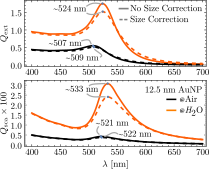
\includegraphics[scale = 1.02]{1-Theory/figs/QextQsca_12-5.pdf}\end{subfigure}
	\hspace*{-.5em}\begin{subfigure}{.05\textwidth}\vspace{-5.5cm}\caption{}\label{sfig:secondaty2}	\end{subfigure}
	\hspace*{-2.em}
	\begin{subfigure}{.48\textwidth} 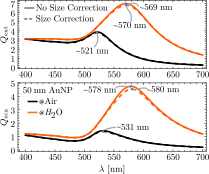
\includegraphics[scale = 1.02]{1-Theory/figs/QextQsca_50.pdf}\end{subfigure}%
\vspace*{-.5em}
\caption[Example of Figure title]{The explanation of your figures. \blindtext}	\label{fig:Main}
\end{figure}

\begin{figure}[h!]\centering
	
\includegraphics[scale=1]{1-Theory/figs/legend.pdf}\\[.5em]
%
	\hspace*{2em}\begin{subfigure}{.05\textwidth}\caption{}\label{sfig:secondary1}\vspace*{6.35cm}\end{subfigure}
	\hspace*{-3.50em}
	\begin{subfigure}{.24\textwidth} 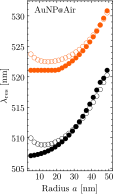
\includegraphics[scale = 1]{1-Theory/figs/redShift_rad1.pdf}\end{subfigure}
%
	\hspace*{.25em}\begin{subfigure}{.05\textwidth}\vspace{-6.35cm}\caption{}\label{sfig:secondaty2}	\end{subfigure}
	\hspace*{-2.5em}
	\begin{subfigure}{.24\textwidth} 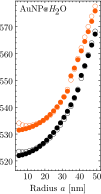
\includegraphics[scale = 1]{1-Theory/figs/redShift_rad2.pdf}\end{subfigure}%
%
	\hspace*{-.5em}\begin{subfigure}{.05\textwidth}\vspace{-6.35cm}\caption{}\label{sfig:secondaty2}	\end{subfigure}
	\hspace*{-2.45em}
	\begin{subfigure}{.24\textwidth} 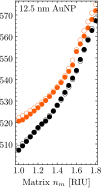
\includegraphics[scale = 1.02]{1-Theory/figs/redShift_mat1.pdf}\end{subfigure}%
%
	\hspace*{-.45em}\begin{subfigure}{.05\textwidth}\vspace{-6.35cm}\caption{}\label{sfig:secondaty2}	\end{subfigure}
	\hspace*{-2.45em}
	\begin{subfigure}{.24\textwidth} 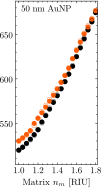
\includegraphics[scale = 1.02]{1-Theory/figs/redShift_mat2.pdf}\end{subfigure}%
\vspace*{-.5em}
\caption[Example of Figure title]{The explanation of your figures. \blindtext}
\label{fig:Main}
\end{figure}


	\section{Mie Scattering}
	\label{section:Mie}

In the previous section, it was concluded that the extinction of light due to the interaction between a particle and a monochromatic plane wave can be determinated through the amplitude of the scattered field in the forward direction. This is stated in the Optical Theorem, which is an exact relation, but inaccuracies can arise when either the scattering amplitude matrix or extinction cross section is approximated\footnote{See for example Section 2.4 from Ref. \cite{tsang_scattering_2000} on the Rayleigh Scattering and Section 21.7 from Ref. \cite{zangwill_modern_2013} on Thompson scattering.}. A particular case in which the scattering amplitude matrix can be exactly calculated is when the scatterer has spherical symmetry. In order to address this special case it will be introduced a vectorial basis with spherical symmetry, known as the Vector Spherical Harmonics (VSH)\index{Scattering!Thompson}\index{Scattering!Rayleigh}\index{Spherical!Vector Spherical Harmonics}. Once the SVH are defined, they will be used to write a monochromatic plane wave and, lastly, the scattered field by a spherical particle will be calculated by imposing the continuity of the tangential components of the electric and magnetic field.

	\subsection{Vector Spherical Harmonics}
		\label{ssection:VSH}		
		% !TeX root = ../tesis.tex

The electric and magnetic field, denoted as $\vb{E}$ and $\vb{B}$, respectively, are a solution to the homogeneous vectorial Helmholtz\index{Helmholtz!Equation, Vectorial} when an harmonic time dependence and a spacial domain with no external charge nor current densities is assumed, that is,
%
% -----------------------------
\begin{subequations}
\begin{tcolorbox}[title = Vectorial Helmholtz Equation,	ams align, breakable]
	\grad^2 \vb{E}(\vb{r},\omega) + k_\text{m}^2 \vb{E}(\vb{r},\omega) &= \vb{0},\\
  \grad^2 \vb{B}(\vb{r},\omega) + k_\text{m}^2 \vb{B}(\vb{r},\omega) &= \vb{0}.
\end{tcolorbox}
\label{eq:Helmholtz}
\end{subequations}
% ------------------------------
%
\noindent where the vectorial operator $\grad^2$ must be understood as $\grad^2 = \nabla(\nabla\cdot) - \nabla\times\nabla\times $, and $k_\text{m}$ is the wave number in the matrix. It is possible to build a basis set for the electric and magnetic fields as long as the elements of this basis are also solution to Eq. \eqref{eq:Helmholtz}. One alternative is to employ the following set of vector functions
%
% -----------------------------
\begin{subequations}
\begin{align}
	\vb{L} =& \nabla \psi,
	\label{eq:L}\\
	\vb{M} =& \nabla\times(\vb{r}\psi),
	\label{eq:M}\\
	\vb{N} =&  \frac{1}{k_\text{m}}\nabla\times\vb{M},
	\label{eq:N}
\end{align}
\label{eq:VSH}
\end{subequations}
% ------------------------------
%
that are solution to the homogeneous vectorial Helmholtz equation as long as the scalar function $\psi$ is solution to the scalar Helmholtz equation\footnote{%
	This result can be proven by considering the following: Let $f$ be $\mathcal{C}^3$ and $\vb{F}$ a $\mathcal{C}^2$. Then, it is true that $\nabla^2(\nabla f) = \nabla(\nabla^2 f)$, and $\curl(\grad^2\vb{F}) = \grad^2(\curl\vb{F})$. }\index{Helmholtz!Equation, Scalar}
%
% -----------------------------
\begin{align}
	\nabla^2 \psi + k_\text{m}^2 \psi = 0.
\label{eq:HelmoltzScalar}
\end{align}
% ------------------------------
%
The triad $\left\{\vb{L},\vb{M},\vb{N}\right\}$ is a set of orthogonal vectors\footnote{%
	Employing the Einstein sum convention with $\epsilon_{ijk}$ the Levi-Civita symbol, Eq. \eqref{eq:M} can be the written as follows:%
	 	$M_i = [\nabla\times(\vb{r}\psi)]_i
	 	=  \epsilon_{ijk}\partial_j(r_k\psi)
	 	=\psi\epsilon_{ijk}\partial_j(r_k) -\epsilon_{ikj}r_k\partial_j\psi
	 	=\psi[\nabla\times\vb{r}]_i - [\vb{r}\times\nabla\psi]_i
	 	= - [\vb{r}\times\nabla\psi]_i
	 	= [\vb{L}\times\vb{r}]_i$,%
	 therefore $\vb{M}$ is orthogonal to $\vb{L}$ and $\vb{r}$. From Eq. \eqref{eq:N} $\vb{M}\cdot\vb{N}=0$.
	 \textcolor{red}{Falta probar $\vb{L}\cdot\vb{N} = 0$.}
	}%
that obey Helmholtz equation \textit{i.e.}, they can be directly identify as electric or magnetic fields. The the elements of the vector basis from Eq. \eqref{eq:VSH}   are known as the Vectorial Spherical Harmonics (VSH) as defined by  \citeauthor{stratton_electromagnetic_2012} \cite{stratton_electromagnetic_2012}, and \citeauthor{bohren_absorption_1983} \cite{bohren_absorption_1983}. The scalar function $\psi$ is known as the generating function of the VSH.


If spherical coordinates are chosen, and it is assume that $\psi(r,\theta,\varphi) = R(r)\Theta(\theta)\Phi(\varphi)$, then Eq. \eqref{eq:HelmoltzScalar} can be decouple into three ordinary differential equations:
%
% ------------------------------
 \begin{align}
	\frac{1}{\Phi}\pdv[2]{\psi}{\varphi} &+ m^2 \Phi =0,
 \label{eq:Phi}\\
	\frac{1}{\sin\theta}\dv{\theta}\qty(\sin\theta\dv{\Theta}{\theta}) &+ \qty[\ell(\ell+1)- \frac{m^2}{\sin^2\theta}]\Theta =0,
	\label{eq:Theta}\\
	\dv{r}\qty(r^2\dv{R}{r}) &+ \qty[ (k_\text{m} r)^2 - \ell (\ell +1)] R =0,
 \label{eq:Req}
\end{align}	
% ------------------------------
%
where $\ell$ can takes natural values and zero, and $\abs{m}\leq \ell$ so $\Phi$ and $\Theta$ are univaluated and finite on a sphere. Eqs. \eqref{eq:Theta} and \eqref{eq:Req} can be rewritten as
%
% ------------------------------
 \begin{align}
(1-\mu^2)\dv[2]{\Theta}{\mu} - 2\mu\dv{\Theta}{\mu} + \qty[\ell(\ell+1)-\frac{m^2}{1-\mu^2}]\Theta &= 0, \qqtext{ with $\mu = \cos\theta$,}
	\label{eq:ThetaMu}\\
	\rho\dv{\rho}\qty(\rho\dv{Z}{\rho}) +  \qty[\rho^2 - \qty(\ell + \frac12)^2]Z  &= 0,  \qqtext{ with $Z = R\sqrt{\rho}$ and $\rho = k_\text{m}r$.}
\label{eq:Reqkr}
\end{align}	
% ------------------------------
%
The solution to Eq. \eqref{eq:ThetaMu} are the Legendre Associated Functions $ P_\ell^m(\mu)$ and to Eq. \eqref{eq:Reqkr} the solution is given by the Spherical Bessel Functions $z_\ell = j_\ell, y_\ell$. Following the convention from most literature on Mie Scattering \cite{zangwill_modern_2013}, the solution to Eq. \eqref{eq:Phi} will be decompose in an odd ($o$) and an even ($e$) solution, that is, as sine and cosine functions. After this procedure, it is determined that the generating function of the VSH is given by
%
% -----------------------------
\begin{subequations}
\begin{tcolorbox}[title = $\psi$: Generating function of the vectorial spherical harmonics,	ams align, breakable]
	\psi_{e\ell m}(r,\theta,\varphi) =& \cos(m\varphi)P_\ell^m(\cos\theta)z_\ell(k_\text{m}r), 
	\\ 	
	\psi_{o\ell m}(r,\theta,\varphi) =& \sin(m\varphi)P_\ell^m(\cos\theta)z_\ell(k_\text{m}r).
\end{tcolorbox}
\label{eq:Helmholtz}
\end{subequations}
% ------------------------------
%
\noindent

























	\subsection{Incident, Scattered and Internal Electric Field}
	\label{ssection:Fields}
		\label{ssection:Fields}
		% !TeX root = ../tesis.tex

 Let $\vb{E}_{0,x}$ be a plane wave traveling in the vertical direction $\vb{e}_z$; its representation in the canonical spherical basis is
 %
 \begin{align}
 \vb{E}_{0,x} (\vb{r})= E_0\qty(\sin\theta\cos\varphi \vu{e}_r +
					\cos\theta\cos\varphi \vu{e}_\theta +
					- \sin\varphi \vu{e}_\varphi) \exp(ikr\cos\theta).
	\label{eq:ExPlane}
 \end{align}
 %
The monochromatic plane wave is a transversal wave, thus it can be written in terms of only the VSH $\vb{M}^{(1)}$ and $\vb{N}^{(1)}$, where the radial dependency is given by $j_\ell$ since the monochromatic plane wave is finite everywhere. Even more, due to the dependency on $\varphi$, it is only restricted to values of $m = 1$. By inspection on the radial component of $\vb{E}_{0,x}$, proportional to $\cos\varphi$ it depends only on $\vb{N}_{e1\ell}^{(1)}$, and on the azimuthal component, proportional to $\sin\varphi$, it can depend on $\vb{M}_{o1\ell}^{(1)}$. Thus, Eq. \eqref{eq:ExPlane} can be written as the linear combination
 %
 \begin{align}
 \vb{E}_{0,x} (\vb{r})= \sum_\ell\qty(a_\ell \vb{M}_{o1\ell}^{(1)} + b_\ell \vb{M}_{e1\ell}^{(1)}).
	\label{eq:ExPlane}
 \end{align}
 %





























































































	\subsection{Au Spherical NPs }
		 \label{ssection:AuMie}
		 % !TeX root = ../tesis.tex

\textbf{Falta emplear las relacinoes de ortogonalidad para calcular las secciones de extincion y edmás}
\clearpage


In Fig. \ref{fig:Mieefficiencies} the extinction  $Q_\text{ext}$ and the scattering  $Q_\text{sca}$ efficiencies of a 12.5 nm AuNP are shown as function of the wavelength $\lambda$ of the incident planewave illuminating the NP. Two matrices were considered in Fig. \ref{fig:Mieefficiencies}: a matrix with a refractive index $n_\text{mat} = 1$ (black lines) modelling air and a matrix with a refractive index $n_\text{mat} = 1.33$ (orange lines) modelling water in the visible spectrum ( $450\text{ nm} < \lambda < 750 \text{ nm}$).  The experimental dielectric function for Au reported by \citeauthor{johnson_optical_1972} \cite{johnson_optical_1972}  was employed to model the electromagnetic response of the spherical AuNP nevertheless, this data corresponds to a bulk sample, meaning that it may not reproduce the optical behavior of a NP since surface effects cease to be neglectable  due to their spacial dimensions \cite{noguez_surface_2007}.   In order to study  the optical properties of AuNP while considering  surface effects,  a size correction to the dielectric function was performed as described in Appendix \ref{app:SizeCorrection}. The efficiencies of the 12.5 nm AuNP  taking into account a dielectric function with (dashed lines) and without (solid lines) a size correction were compared for both considered matrices; on each curve the wavelength of their maximum value, which corresponds to the wavelength of the LSPR, is indicated.


 
\begin{figure}[h!]
	\def\svgwidth{1\textwidth} \small
\vspace*{3.25em}
\hspace*{-10.75em}
\begin{subfigure}{.49\textwidth}\caption{ }\label{fig:Mieefficiencies:a}\end{subfigure}
\begin{subfigure}{.49\textwidth}\caption{ }\label{fig:Mieefficiencies:b}\end{subfigure}
\vspace*{-6.25em}\\
\includeinkscape{1-Theory-Figs/Mie-Au/1-Efficiencies}
\vspace*{-2em}
\caption[Extinction and Scattering Corss Section of a 12.5 nm Au spherical NP embeded into a vacuum- and into a waterlike environment]{ \textbf{a)} Extinction $Q_\text{ext}$ and \textbf{b)} Scattering $Q_\text{sca}$ a Efficiencies of a 12.5 nm Au spherical NP embeded into a vacuum-like matrix (black, $n_\text{mat} = 1$)  and into a water-like matrix (orange, $n_\text{mat} = 1.33$), as function of  the wavelength $\lambda$ of the incident plane wave.  The solid curves were calculated by considering no size effects on the dielectric function of the AuNP, while the dashed curves considers a size correction to it; the experimental data of \citeauthor{johnson_optical_1972} \cite{johnson_optical_1972} was employed.} 
\label{fig:Mieefficiencies} 
\end{figure}
 
From the extinction and scattering efficiencies in Fig. \ref{fig:Mieefficiencies}, two main spectral tendencies arises between these quantities: on the overall value of the efficiencies and on the spectral position of their maximum. Since the scattering efficiency is two orders of magnitude smaller than the extinction efficiency within the visible range, the main energy loss mechanism is absorption, as stated by the Optical Theorem [Eq. \eqref{eq:Cext}]. Even though the 12.5 nm AuNP absorbs more light than what it scatters, both phenomena are present. For example, when the  studied AuNP is embedded in air, the wavelengths at which it absorbs and scatters the most are $\sim 509$ nm and $\sim 522$ nm, respectively. When the AuNP is embedded into water, the absorption of light is optimized at a wavelength of $\sim 525$ nm, while the scattering is optimized at $\sim 533$ nm. For both an air and a water matrix, the wavelength of most scattering is $\sim 10$ nm redshifted relative to the wavelength of most absorption. As it can be seen, the extinction and scattering may have different spectral tendencies as already discussed, yet they share common characteristics   when the dependency on the embedding media or on the size of the particle are studied.

The scattering and the absorption efficiencies of a 12.5 nm AuNP present an overall increase within the visible range when the refractive index of the matrix, the embedding media,  increases. This can be seen by comparing the black curves ($n_\text{mat} = 1$) with the orange curves ($n_\text{mat} = 1.33$), which are at least 
 

 

 
 
 
\begin{figure}[h!]
	\def\svgwidth{1\textwidth} \small
\vspace*{3.25em}
\hspace*{-6.5em}
\begin{subfigure}{.49\textwidth}\caption{$\norm{S_{1,2}(\theta)}^2\times 10^5$}\label{fig:Mieefficiencies:a}\end{subfigure}
\begin{subfigure}{.49\textwidth}\caption{$\norm{S_{1,2}(\theta)}^2\times 10^4$}\label{fig:Mieefficiencies:b}\end{subfigure}
\vspace*{-6.25em}\\
\includeinkscape{1-Theory-Figs/Mie-Au/2-ScatteringMaps}
\vspace*{-2em}
\caption[Extinction and Scattering Corss Section of a 12.5 nm Au spherical NP embeded into a vacuum- and into a waterlike environment]{ \textbf{a)} Extinction $Q_\text{ext}$ and \textbf{b)} Scattering $Q_\text{sca}$ a Efficiencies of a 12.5 nm Au spherical NP embeded into a vacuum-like matrix (black, $n_\text{mat} = 1$)  and into a water-like matrix (orange, $n_\text{mat} = 1.33$), as function of  the wavelength $\lambda$ of the incident plane wave.  The solid curves were calculated by considering no size effects on the dielectric function of the AuNP, while the dashed curves considers a size correction to it; the experimental data of \citeauthor{johnson_optical_1972} \cite{johnson_optical_1972} was employed.} 
 \end{figure}




\chapter{The Finite Element Method}
\label{chapter:FEM}



	\section{Finite Element Method and Analytical Solutions}
		\label{sec:FEM-Mie}
		% !TeX root = ../tesis.tex

%
\begin{figure}[h!]\centering
	\def\svgwidth{.8\textwidth} \small
\includeinkscape{SistemaMie}
\vspace*{0em}
\caption[Spherical symmetric COMSOL Setup]{A 3D view (left) and the cross section (right) of a spherical symmetric COMSOL setup to calculate the optical response of a single spherical NP embedded into a matrix. The NP (yellow) is located at the center of the matrix (gray), which is covered by a PML layer (blue). The upper layer of the PML is hidden to allow a better view of the setup.}
\label{fig:setup:sphere}
\end{figure}


%
\begin{figure}[h!]
\def\svgwidth{\textwidth} \small
\hspace*{.75em}
\begin{subfigure}{.1\textwidth}\caption{ }\label{fig:Eff:sphere:First:a}\end{subfigure}
\vspace*{12.5em} % Crece la distancia entre as etiquetas
\\
\vspace*{-16.5em} % Crece la distancia entre las etiquetas y el pie de figura
\hspace*{0.5em}%
\begin{subfigure}{.1\textwidth}\caption{ }\label{fig:Eff:sphere:First:b}\end{subfigure}\\
\includeinkscape{1-Theory-Figs/0-NoConv}
\vspace*{-1.5em} %Crece la ditancia entre la imagen y el pie de figura
\caption[Scattering, Absorption and Extinction Efficiencies of a 5 nm AuNP$@$Air: Analytical and FEM solutions with no optimizatio]{\textbf{a)} Scattering $Q_\text{sca}$, absorption $Q_\text{abs}$ and extinction $Q_\text{ext}$ efficiencies of a 5 nm AuNP embedded into air calculated by means of the Mie Theory (continuous) and the FEM (disks), and \textbf{b)} their absolute error, as function of the wavelength $\lambda$ of the incident planewave. The chosen parameters for the FEM calculations were based on the COMSOL Excercises \textbf{CITAR}.}
\label{fig:Eff:sphere:First}
\end{figure}


%
\begin{figure}[h!]\centering
	\def\svgwidth{.8\textwidth} \small
\includeinkscape{1-Theory-Figs/1-RadiusConv}
\vspace*{-1em}
\caption[Extinction Efficiency Absolute Error: NP Max Mesh Size Analysis]{Absolute error between the Mie Theory and the FEM calculation on the extinction efficiency $Q_\text{ext}$ of a 5nm AuNP$@$Air as function of the maximum mesh size within the NP at the wavelength of the LSPR.}
\label{fig:Eff:sphere:radius}
\end{figure}

%
\begin{figure}[h!]\centering
	\def\svgwidth{.8\textwidth} \small
\includeinkscape{1-Theory-Figs/2-MatrixConv}
\vspace*{-1em}
\caption[Extinction Efficiency Absolute Error: Matrix Max Mesh Size Analysis]{Absolute error between the Mie Theory and the FEM calculation on the extinction efficiency $Q_\text{ext}$ of a 5nm AuNP$@$Air as function of the maximum mesh size within the matrix at the wavelength of the LSPR.}
\label{fig:Eff:sphere:matrix}
\end{figure}


\begin{figure}[h!]\centering
	\def\svgwidth{.8\textwidth} \small
\includeinkscape{1-Theory-Figs/3-MatrixPMLThickness}
\vspace*{-1em}
\caption[Extinction Efficiency Absolute Error: Matrix and PML Thickness Analysis]{Absolute error between the Mie Theory and the FEM calculation on the extinction efficiency $Q_\text{ext}$ of a 5nm AuNP$@$Air as function of the matrix thickness (black) and the PML thickness (orange) at the wavelength of the LSPR. It wac chosen for both cases a NP maximum mesh size of $a/10$ and a matrix maximum mesh size of $\lambda/6$; the default thickness of the matrix and PML was set to $\lambda/4$.}
\label{fig:Eff:sphere:thickness}
\end{figure}








%
%
%
%\begin{figure}\centering
%%\def\svgwidth{\textwidth} \small
%%\includeinkscape{2-Results-Figs/redshift/redshift}%
%\includegraphics[width = .8\textwidth ]{1-Theory-Figs/Mie-FEM_Air.pdf}\\
%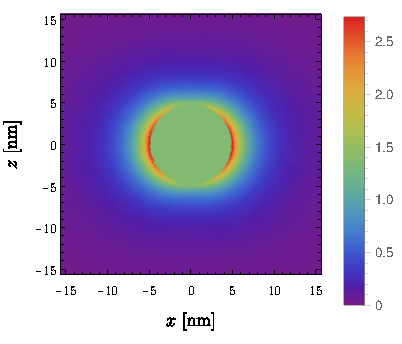
\includegraphics[width = .4\textwidth ]{1-Theory-Figs/Isolated-COMSOL.pdf}%
%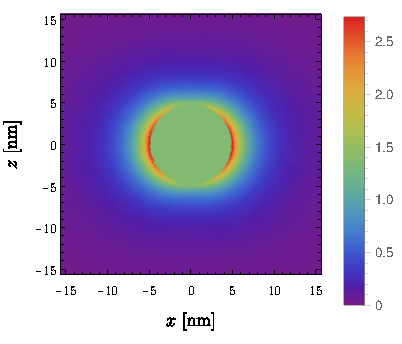
\includegraphics[width = .4\textwidth ]{1-Theory-Figs/Isolated-COMSOL.pdf}%
%\caption[Convergence tests: The Meshing]{Resonance wavlength ($\lambda_\text{res}$) of the scattering (orange) and extinction (black) cross sections as functions of the NPs radii when embedded  \ref{sfig:red:1} into air and \ref{sfig:red:2} into water, and as function of the refractive index of the matrix for NP of radius set to  \ref{sfig:red:3} 12.5 nm and \ref{sfig:red:4} 50 nm.}
%\end{figure}




\begin{figure}[h!]\centering
	\def\svgwidth{.8\textwidth} \small
\includeinkscape{1-Theory-Figs/SistemaBox}
\vspace*{0em}
\caption[Spherical symmetric COMSOL Setup]{A 3D view (left) and the cross section (right) of a spherical symmetric COMSOL setup to calculate the optical response of a single spherical NP embedded into a matrix. The NP (yellow) is located at the center of the matrix (gray), which is covered by a PML layer (blue). The upper layer of the PML is hidden to allow a better view of the setup.}
\label{fig:setup:sphere}
\end{figure}

\begin{figure}[h!]
\def\svgwidth{\textwidth} \small
\hspace*{-1.25em}
\begin{subfigure}{.1\textwidth}\caption{ }\label{fig:Eff:sphere:First:a}\end{subfigure}
\vspace*{12.5em} % Crece la distancia entre as etiquetas
\\
\vspace*{-16.5em} % Crece la distancia entre las etiquetas y el pie de figura
\hspace*{-.75em}%
\begin{subfigure}{.1\textwidth}\caption{ }\label{fig:Eff:sphere:First:b}\end{subfigure}\\
\includeinkscape{1-Theory-Figs/4-Conv}
\vspace*{-1.5em} %Crece la ditancia entre la imagen y el pie de figura
\caption[Scattering, Absorption and Extinction Efficiencies of a 5 nm AuNP$@$Air: Analytical and FEM solutions with no optimizatio]{\textbf{a)} Scattering $Q_\text{sca}$, absorption $Q_\text{abs}$ and extinction $Q_\text{ext}$ efficiencies of a 5 nm AuNP embedded into air calculated by means of the Mie Theory (continuous) and the FEM (disks), and \textbf{b)} their absolute error, as function of the wavelength $\lambda$ of the incident planewave. The chosen parameters for the FEM calculations were based on the COMSOL Excercises \textbf{CITAR}.}
\label{fig:Eff:sphere:First}
\end{figure}

		
%

\chapter{Results and Discussion}
	% !TeX root = ../tesis.tex

To compare the optical response of a NP in the presence of a substrate with that of a NP in a totally homogeneous environment, let us first analyze the spectral response given by the Mie Theory when the matrix and the size of the NP varies. In Fig. \ref{fig:Mie:redshift} it is shown the wavelength of resonance $\lambda_\text{res}$, that is, the wavelength at which the scattering (orange) and extinction (black) efficiencies are maximized,  as a  function of the radius $a$ of a AuNP embedded in a matrix of air [Fig. \ref{sfig:red:1}] and of glass [Fig. \ref{sfig:red:2}], with a refractive index of $n_\text{m} = 1$ and $n_\text{m} = 1.5$, respectively, and as a function of the refractive index of the matrix $n_\text{m}$ for a AuNP with a radius of {$a = 12.5$ nm} [Fig. \ref{sfig:red:3}] and with a radius of $a = 50$ nm [Fig. \ref{sfig:red:4}]. For the optical response of the AuNP it was employed the experimental data as reported by \citeauthor{johnson_optical_1972} \cite{johnson_optical_1972} (filled circles) and by considering a size correction ---see Appendix \ref{app:SizeCorrection}--- to it (empty circles).

\begin{figure}[h!]
    \def\svgwidth{\textwidth}
    \includeinkscape[pretex = \small]{Redshift/redshift}
    \vspace*{-20.9em} \\
    \hspace*{1em}%
        \begin{subfigure}{.225\textwidth}\caption{AuNP$@$Air}\label{sfig:red:1}\end{subfigure}%
        \begin{subfigure}{.28\textwidth}\caption{AuNP$@$Glass}\label{sfig:red:2}\end{subfigure}%
        \begin{subfigure}{.225\textwidth}\caption{12.5 nm AuNP}\label{sfig:red:3}\end{subfigure}%
        \begin{subfigure}{.24\textwidth}\caption{50 nm AuNP}\label{sfig:red:4}\end{subfigure}
    \vspace*{16.5em}\\
    \caption[Spectral redshift of the scattering and extinction  efficiencies of a spherical AuNP as a function of its size and the embedding media]{Resonance wavelength $\lambda_\text{res}$ of the scattering (orange) and extinction (black) efficiencies of a AuNP as a function of the NP's radius when embedded \textbf{a)} in air ($n_\text{m} = 1)$ and \textbf{b)} in glass ($n_\text{m} = 1.5$), and as a function of the refractive index of the matrix  $n_\text{m}$ for a AuNP of radius \textbf{c)} 12.5 nm and \textbf{d)} 50 nm, using the dielectric function for gold as reported by \citeauthor{johnson_optical_1972} \cite{johnson_optical_1972} (filled circles) and considering a size correction to it (empty circles).}
    \label{fig:Mie:redshift}
\end{figure}

From the results shown in Fig. \ref{fig:Mie:redshift} it can be seen that the wavelength of resonance  $\lambda_\text{res}$ for the extinction, considering the bulk dielectric function for Au (filled circles), is smaller than that of the scattering  and that the distance between them decreases as either the size of the AuNP or the refractive index of the matrix increases. This behavior arises from a redshift of $\lambda_\text{res}$ for increasing values of $a$ and $n_\text{m}$ and it shows that, for particles small compared to the wavelength of the incident light in the matrix, the main contribution to the extinction of light  is due to absorption processes and as the size of the AuNP grows, the extinction is dominated by its other contribution: the scattering, as discussed in Section \ref{ss:AuMie} and supported by Eq. \eqref{eq:Cext}. The redshift of   $\lambda_\text{res}$ can also be observed when considering a size corrected dielectric function (empty circles). Remarkably, for values of radius $\lesssim 15/n_\text{m}$ there is a blueshift of $\lambda_\text{res}$, as it can be seen in Figs. \ref{sfig:red:1} and \ref{sfig:red:2}, which is a consequence of a greater imaginary part of the dielectric function for the AuNP due to the size correction. On the other hand, an increase in $n_\text{m}$ for a fixed radius presents only redshifts either with or without a size corrected dielectric function [see Figs. \ref{sfig:red:3} and  \ref{sfig:red:4}].

The spectral behavior of the scattering and extinction of light due to a spherical NP summarized in Fig. \ref{fig:Mie:redshift} was calculated by assuming a homogeneous medium (the matrix) where the NP is embedded and thus allowing the direction of the illuminating plane wave to be arbitrary, yet yielding the same results. In the following Sections, the homogeneity of the surroundings of the NP is substituted by two semiinfinite media and thus modifying the optical response of the system depending on how it is illuminated.

	\section{Incrustation Degree of a Spherical Particle}
	% !TeX root = ../tesis.tex


\chapter{Results}

\section{What I got}
\label{section:results}
				
\Blindtext

    \section{Future Work: Application on Metasurfaces}
    
\chapter{Conclusions}


\appendix
\chapter{Size Corrected Dielectric Function}
\label{app:SizeCorrection}
% !TeX root = ../tesis.tex



\begin{figure}
\def\svgwidth{\textwidth} \small
\includeinkscape{5-Apendices-Figs/DrudeFit}%

\caption{   }
\end{figure}









\chapter{Mie Theory (Conventions and Code)}
% !TeX root = ../tesis.tex

The Vector Spherical Harmonics (VSH) where defined in Sec. \ref{ssection:VSH} in terms of their generating function $\psi(r,\theta,\varphi)$ which must satisfy the scalar Helmholtz equation [Eq.  \eqref{eq:HelmoltzScalar}]. By employing the separation of variables method,  it was determined that $\psi$ is the product of either $\sin(m\varphi)$ or $\cos(m\varphi)$, of the associated Legendre functions $P_\ell^m(\cos\theta)$ and the spherical Bessel/Hankel functions $z_\ell(kr)$, all of which are solutions to Eqs. \eqref{eq:Phi}-\eqref{eq:Reqkr}. In this section, it is discussed the chosen definitions for $P_\ell^m$, $z_\ell$ and related functions, as well as how to calculate them. It is also detailed how to code the Mie Theory results employing the Wolfram Language.

\section*{Radial Dependency: Spherical Bessel/Hankel Functions}

The radial dependency of the VSH is given by the two linearly independent solutions to Eq. \eqref{eq:Reqkr} which are the spherical Bessel function of first and second kind $j_\ell(\rho)$ and $y_\ell(\rho)$, respectively, related by the regular Bessel function of fractional order $J_{\ell+1/2}(\rho)$ and  $Y_{\ell+1/2}(\rho)$ by
%
\begin{align}
j_\ell(\rho) = \sqrt{\frac{\pi}{2 \rho}}J_{\ell+1/2}(\rho),\qqtext{ and} 
y_\ell(\rho) = \sqrt{\frac{\pi}{2\rho}}Y_{\ell+1/2}(\rho).
\label{eq:bessel}
\end{align}
%
Another set of two linear independent solutions to  Eq. \eqref{eq:Reqkr} are the spherical Hankel functions  of first ($h^{(1)}_\ell$)  and second kind ($h^{(1)}_\ell$) given by
\begin{align}
h^{(1)}_\ell(\rho) = j_\ell(\rho) + i y_\ell(\rho),\qqtext{ and} 
h^{(2)}_\ell(\rho) = j_\ell(\rho) - i y_\ell(\rho).
\label{eq:Hankel}
\end{align}
%
Since the spherical Hankel functions are a linear combination of the Bessel spherical functions, they four obey the following recurrence relations
%
\begin{align}
\frac{z_\ell(\rho)}{\rho} =& \frac{z_{\ell-1}(\rho) + z_{\ell+1}(\rho)}{2\ell + 1},
\label{eq:recBessel1}\\
\dv{z_\ell(\rho)}{\rho} =& \frac{\ell z_{\ell-1}(\rho) - (\ell+1)z_{\ell+1}(\rho)}{2\ell + 1} ,
\label{eq:recBessel2}
\end{align}
%
with $z_\ell$ any of the functions in Eqs. \eqref{eq:bessel} and \eqref{eq:Hankel}.


\section*{Azimuthal Angular Dependency $\varphi$: Sine, Cosine}

Within this text, it was chosen the azimuthal solution to the scalar Helmholtz equation to be sines and cosines, so $m$ can only take non negative integer values. This functions obey the orthogonality relations
%
\begin{align}
\int_0^{2\pi} \sin(m\varphi)\sin(m'\varphi) \dd{\varphi} &= \delta_{m,m'}( 1 - \delta_{0,m}) \pi,
\label{eq:SinOrth}\\
\int_0^{2\pi} \cos(m\varphi)\cos(m'\varphi) \dd{\varphi} & =\delta_{m,m'}( 1+ \delta_{0,m}) \pi,
\label{eq:CosOrth}\\
\int_0^{2\pi} \cos(m\varphi)\sin(m'\varphi) \dd{\varphi} &=0,
\label{eq:SinCosOrth}
\end{align}
%
with $\delta_{m,m'}$ the Kroneker delta.

\section*{Polar Angular Dependency: Associated Legendre Functions and the Angular Functions $\pi_\ell$ and $\tau_\ell$}
The solution to the polar angle equation are the associated Legendre functions and in this work they are defined as by \citeauthor{arfken_mathematical_2001} \cite{arfken_mathematical_2001}, that is,
%
\begin{equation}
P_\ell^m(\mu) = (1-\mu^2)^{m/2}\dv[m]{\,}{\mu}\hspace*{.05em} P_\ell(\mu),
\qqtext{ with}
P_\ell(\mu) = \frac{1}{2^\ell \ell!}\dv[\ell]{\,}{\mu}\hspace*{.05em}  (\mu^2-1)^\ell ,
\label{eq:Plm}
\end{equation}
%
where $\mu = \cos\theta$ and $P_\ell(\mu)$ are the Legendre polynomials with $\ell$ a non negative integer. With such definition, the  associated Legendre functions follows the orthogonality relation
%
\begin{align}
\int_{-1}^1 P_\ell^m(\mu)P_{\ell'}^m(\mu)\dd{\mu} = \frac{2\delta_{\ell,\ell'}}{2\ell+1}\frac{(\ell+m)!}{(\ell-m)!}.
\label{eq:PlmOrtho}
\end{align}
%
It was shown in Section \ref{ssection:Fields} that the a plane wave can be written as a linear combination of the VSH with only $m = 1$, which lead to the definition of the angular functions $\pi_\ell$ and $\tau_\ell$ given by
%
\begin{align*}
 \pi_\ell(\cos\theta )  = \frac{P_\ell^1(\cos\theta)}{\sin\theta},\qqtext{and}
 \tau_\ell(\cos\theta) = \dv{P_\ell^1(\cos\theta)}{\theta},
\end{align*}
%
which can be calculated recursively with Eq. \eqref{eq:Plm}  and the recurrence relations of the Legendre polynomials
%
\begin{align}
(2\ell-1)\mu P_{\ell-1}(\mu) =& (\ell-1) P_{\ell}(\mu) + \ell P_{\ell-2}(\mu),\\
(1-\mu)^2\dv{P_\ell(\mu)}{\mu} =& \ell P_{\ell-1}(\mu) - \ell\mu P_\ell(\mu).
\end{align}
%
leading to 
%
\begin{align}
\pi_\ell(\mu) =& \frac{2\ell-1}{\ell-1}\mu \pi_{\ell-1}(\mu) - \frac{\ell}{\ell-1}\pi_{\ell-2},\\
\tau_ \ell (\mu) =& \ell\mu\pi_\ell(\mu) - (\ell+1)\pi_{\ell-2}(\mu).
\end{align}
%
where $\pi_1(\mu) = 1$ according to  Eq. \eqref{eq:Plm} and where $\pi_0(\mu)=0$ is defined. Another notable result from Eq. \eqref{eq:Plm} is that the angular functions $\pi_\ell(\mu)$ and $\tau_\ell(\mu)$, when evaluated at $\theta =0$ ($\mu = 1$),  follows 
%
\begin{align}
\pi_\ell(\mu=1) & =  \dv{P_\ell(\mu)}{\mu}\eval_{\mu=1},\\
\tau_\ell (\mu = 1) & = \qty[\dv{P_\ell^1(\mu)}{\mu} + (1-\mu^2)^{1/2}\dv[2]{P_\ell(\mu)}{\mu}]\eval_{\mu=1} = \dv{P_\ell(\mu)}{\mu}\eval_{\mu=1},
\end{align}
%
which can be obtained from the Legendre equation  by setting $m = 1$ and $\mu = 1$ in Eq. \eqref{eq:ThetaMu}, leading to
%
\begin{align}
\pi_\ell(\mu=1) = \tau_\ell(\mu=1) = \frac{\ell(\ell+1)}{2} P_\ell(\mu = 1) = \frac{\ell(\ell+1)}{2},
\label{eq:PiTau0}
\end{align}
%
where the last equality arises from the chosen definition of the Legendre polynomial [Eq. \eqref{eq:Plm}].

The angular functions $\pi_\ell$  and $\tau_\ell$ are not orthogonal in general, nevertheless  $\pi_\ell(\mu)\pm\tau_\ell(\mu)$ are. To prove the orthogonality of $\pi_\ell\pm\tau_\ell$ let us apply the Legendre equation [Eq. \eqref{eq:Theta}] to $P_\ell^m$ and multiply it by $P_{\ell'}^m$; repeating this procedure inverting $\ell$ and $\ell'$ and adding both equations it is obtained that
%
\begin{align}
\dv{\theta}&\qty(\sin\theta P_{\ell'}^m(\mu)\dv{P_\ell^m(\mu)}{\theta}) +
\dv{\theta}\qty(\sin\theta P_{\ell}^m(\mu)\dv{P_{\ell'}^m(\mu)}{\theta}) +  
\label{eq:PlPl'}
\\
&\qty[\ell(\ell+1)+\ell'(\ell'+1)]P_{\ell'}^m(\mu)P_{\ell}^m(\mu) \sin\theta
=
 2\qty(\frac{mP_\ell^m(\mu)}{\sin\theta}\frac{mP_{\ell'}^m(\mu)}{\sin\theta}+ \dv{P_\ell^m(\mu)}{\theta}\dv{P_{\ell'}^m(\mu)}{\theta})\sin\theta,\notag
\end{align}
%
where  it was added $2\dv*{P_\ell^m}{\theta}\dv*{P_{\ell'}^m}{\theta}$ on both sides to complete the derivatives. Integrating Eq. \eqref{eq:PlPl'} in th interval $\theta \in (0,\pi)$, or $\mu \in(-1,1)$, and employing Eqs. \eqref{eq:Plm} and \eqref{eq:PlmOrtho}, one obtains that
%
\begin{align}
\int_{-1}^1 \qty(\frac{mP_\ell^m(\mu)}{\sin\theta}\frac{mP_{\ell'}^m(\mu)}{\sin\theta}+ \dv{P_\ell^m(\mu)}{\theta}\dv{P_{\ell'}^m(\mu)}{\theta})\dd{\mu} = 
\delta_{\ell,\ell'}\frac{2\ell(\ell+1)}{2\ell+1}\frac{(\ell+m)!}{(\ell-m)!}.
\label{eq:PimlTauml}
\end{align}
%
Additionally 
%
\begin{align}
\int_{-1}^1\frac{mP_\ell^m(\mu)}{\sin\theta}\dv{P_{\ell'}^m(\mu)}{\theta}\dd{\mu}
 = \int_0^{\pi} mP_\ell^m(\mu)\dv{P_{\ell'}^m(\mu)}{\theta}\dd{\theta} = 
 -\int_{-1}^1\frac{mP_{\ell'}^m(\mu)}{\sin\theta}\dv{P_{\ell}^m(\mu)}{\theta}\dd{\mu}.
 \label{eq:taupiCross}
\end{align}
%
where Eq. \eqref{eq:Plm} was employed along integration by parts. Thus, combining Eqs. \eqref{eq:PimlTauml} and \eqref{eq:taupiCross}, it leads to
%
\begin{align}
\int_{-1}^{1}\qty(\frac{mP_\ell^m(\mu)}{\sin\theta}\pm\dv{P_\ell^m(\mu)}{\theta})\qty(\frac{mP_{\ell'}^m(\mu)}{\sin\theta}\pm\dv{P_{\ell'}^m(\mu)}{\theta})\dd{\mu}  
 =  \delta_{\ell,\ell'}\frac{2\ell(\ell+1)}{2\ell+1}\frac{(\ell+m)!}{(\ell-m)!}.
 \label{eq:(pipmtau)}
\end{align}
%
The Eq. \eqref{eq:(pipmtau)}  is the orthogonality of $\pi_\ell(\mu)\pm\tau_\ell(\mu)$ when $m = 1$, which also simplifies the right hand side to $\delta_{\ell,\ell'} 2\ell^2(l+1)^2/(2\ell+1)$.


\section*{Vector Spherical Harmonics Orthogonality Relations}

The VSH follow orthogonality relations inherited from the orthogonality of sine, cosine and the associated Legendre functions. Let us define the inner product as the integral in the solid angle between two vector functions as 
%
\begin{align}
\ev{\vb{A},\vb{A}'}_\Omega = \int_0^{2\pi}\int_0^{\pi} \vb{A}\cdot\vb{A}'\sin\theta\dd{\theta}\dd{\varphi}.
\label{eq:inner}
\end{align}
%
Under this inner product, all even VSH are orthogonal to the odd VSH, as well as all VSH  with $m\neq m', $due to the orthogonality of $\sin(m\varphi)$ and $\cos(m'\varphi)$. The remaining orthogonality relations  can be obtained by employing Eq. \eqref{eq:PimlTauml}, leading to 
%
\begin{align}
&\ev{\vb{L}_{em'\ell},\vb{L}_{em'\ell'}}_\Omega = \ev{\vb{L}_{om\ell},\vb{L}_{om\ell'}}_\Omega \notag\\
	 &\hspace*{2em} =  
 	\delta_{m,m'}\delta_{\ell,\ell'} (1\pm\delta_{m,0}) 
 	\frac{2\pi}{2\ell+1}\frac{(\ell+m)!}{(\ell-m)!}
 	\qty[\qty(k\dv{z_\ell(kr)}{(kr)})^2 + \ell(\ell+1)\qty(k\frac{z_\ell(kr)}{kr})^2],\\
%
&\ev{\vb{M}_{em\ell},\vb{M}_{em\ell'}}_\Omega = \ev{\vb{M}_{om\ell},\vb{M}_{om\ell'}}_\Omega \notag\\
		 &\hspace*{2em} =  
	\delta_{m,m'}\delta_{\ell,\ell'} (1\pm\delta_{m,0}) 
	\pi \frac{2  \ell(\ell+1)}{2\ell+1}\frac{(\ell+m)!}{(\ell-m)!}
	z_{\ell}^2(kr),\\
%
&\ev{\vb{N}_{em\ell},\vb{N}_{em\ell'}}_\Omega = \ev{\vb{N}_{om\ell},\vb{N}_{om\ell'}}_\Omega  \notag\\
	 &\hspace*{2em} =  
	 \delta_{m,m'}\delta_{\ell,\ell'} (1\pm\delta_{m,0}) 
	\pi \frac{2  \ell(\ell+1)}{2\ell+1}\frac{(\ell+m)!}{(\ell-m)!}
	\qty[\qty(\frac{ z_{\ell}}{kr})^2 + \qty(\frac{1}{kr}\dv{[kr z_\ell(kr)]}{(kr)})^2]. \\
%%
&\ev{\vb{L}_{em\ell},\vb{N}_{em\ell'}}_\Omega = \ev{\vb{L}_{om\ell},\vb{N}_{om\ell'}}_\Omega \notag\\
	 &\hspace*{2em} =
	 \delta_{m,m'}\delta_{\ell,\ell'} (1\pm\delta_{m,0}) 
	\pi \frac{2  \ell(\ell+1)}{2\ell+1}\frac{(\ell+m)!}{(\ell-m)!}
	\qty[\frac{ z_{\ell}}{kr}\dv{z_\ell(kr)}{(kr)} + \qty(\frac{1}{kr}\dv{[kr z_\ell(kr)]}{(kr)})^2]
\end{align}
%
where $(1+\delta_{m,0}) $ is for odd VSH and $(1-\delta_{m,0}) $ for even VSH. The orthogonality relations of the VSH can be further simplify by means of the recurrence relations of the spherical Bessel/Hankel functions [Eqs. \eqref{eq:recBessel1} and \eqref{eq:recBessel2}], which imply that
%
\begin{align}
\qty[\qty(k\dv{z_\ell(kr)}{(kr)})^2 + \ell(\ell+1)\qty(k\frac{z_\ell(kr)}{kr})^2] =& k^2 
		\qty[\ell z_{\ell-1}^2(kr) + \ell(\ell+1)z_{\ell+1}^2(kr)],\\
\qty[\qty(\frac{ z_{\ell}}{kr})^2 + \qty(\frac{1}{kr}\dv{[kr z_\ell(kr)]}{(kr)})^2] =&
 	\ell(\ell+1)\qty[(\ell+1) z_{\ell-1}^2(kr)+ \ell z_{\ell+1}^2(kr)],  \\	
\qty[\frac{ z_{\ell}}{kr}\dv{z_\ell(kr)}{(kr)} + \qty(\frac{1}{kr}\dv{[kr z_\ell(kr)]}{(kr)})^2] =&
	 	\ell(\ell+1)\qty[z_{\ell-1}^2(kr)- z_{\ell+1}^2(kr)].	
\end{align}
%



\section*{Mie Theory Code}
%
%{\footnotesize
%\begin{mmaCell}[
%	pattern = {n, th,n_,th_,i},
%	local = {pi}
%	]{Code}
%  (*Angular functions pi and tau - n-> order - th -> polar angle theta*)
%  MiePi[n_, th_] := Module[{pi}, 
%     pi[0] = 0; pi[1] =  1;  
%     pi[\mmaPat{i_}] := pi[i] = ((2i-1)/(i-1)) * Cos[th] * pi[i-1] - (i/(i-1)) * pi[i-2]; 
%    pi[n]]
%     
%  MieTau[n_, th_] := Module[{pi}, 
%     pi[0] = 0; pi[1] = 1;  
%     pi[\mmaPat{i_}] := pi[i] = ((2i-1)/(i-1)) * Cos[th] * pi[i-1] - (i/(i-1)) * pi[i-2]; 
%    n * Cos[th] * pi[n] - (n+1) * pi[n-1]]
%
%		SetAttributes[MiePi, Listable]
%		SetAttributes[MieTau, Listable]
%\end{mmaCell}
%}
%{\footnotesize
%\begin{mmaCell}[
%	pattern = {n_, x_, m_, n, x, m, \#},
%	local = {an, bn, psiMX, dpsiMX, psiX, dpsiX, xiX, dxiX}
%	]{Code}	
%  MieCoefficient[n_, x_, m_] := 
%   Module[{an, bn, psiMX, dpsiMX, psiX, dpsiX, xiX, dxiX},
%    If[! Apply[Equal, Length /@ {x, m, 0}], 
%    Return[Message[MieCoefficient::list, x, m]]];
%  
%   {psiMX, dpsiMX} = 
%     {m*x*#, -n*# + m*x*SphericalBesselJ[n-1, m*x]} &@ SphericalBesselJ[n, m*x];
%   {psiX, dpsiX} = 
%     {x*#, -n*# + x*SphericalBesselJ[n - 1, x]} &@ SphericalBesselJ[n, x];
%   {xiX, dxiX} = {psiX, dpsiX} + 
%      I*{x*#, -n*# + x*SphericalBesselY[n-1, x]} &@ SphericalBesselY[n, x];
%  
%  an = (m*psiMX*dpsiX - psiX*dpsiMX)/(m*psiMX*dxiX - xiX*dpsiMX);
%  bn = (psiMX*dpsiX - m*psiX*dpsiMX)/(psiMX*dxiX - m*xiX*dpsiMX);
%  
%  {an, bn}]
%\end{mmaCell}
%}
%
%{\footnotesize
%\begin{mmaCell}[
%	pattern = {x_, m_, x, m, angle_, angle, \#},
%	local = {ab, poles, pitau, coeff,  s1, s2}
%	]{Code}	
%  MieScatteringAmplitude12[x_, m_, angle_] :=  
%   Module[{ab, poles, pitau, coeff,  s1, s2},
%   
%   (*Wacombe criteria for convergence*)
%   poles = Range[ Ceiling[ x + 4.*x^(1./3) + 2.]];
%  
%   ab = MieCoefficient[poles, x, m];
%   pitau = Through[{MiePi, MieTau}[poles, angle]];
%   coeff = ((2.*# + 1.)/((# + 1.)*#)) & /@ poles;
%  
%   s1 = Plus @@ (coeff * Plus @@ (ab*pitau));
%   s2 = Plus @@ (coeff * Plus @@ (ab* Reverse[pitau]));
%  
%  {s1, s2}]
%\end{mmaCell}
%}
%
%{\footnotesize
%\begin{mmaCell}[
%	pattern = {indices_, wlength_, radius_, indices, wlength, radius, \#},
%	local = {ab, sum, x, poles}
%	]{Code}	
%  MieScatteringQ[indices_, wlength_, radius_] := 
%   Module[{ab, sum, x, poles},
%    x = (2.*Pi*radius)*indices[[1]]/wlength; (*Size parameter*)
%    (*Wacombe criteria for convergence*)
%    poles = Range[ Ceiling[ x + 4.*x^(1./3) + 2.]]; 
%    
%    ab = Plus @@ ( Chop[#*Conjugate[#]] &@ 
%    		 MieCoefficient[poles, x, Divide @@ Reverse[indices]]);
%    sum = Plus @@ ((2.*# + 1 & /@ poles) * ab);
%   sum *= 2./(x^2)]
%\end{mmaCell}
%}
%
%{\footnotesize
%\begin{mmaCell}[
%	pattern = {indices_, wlength_, radius_, indices, wlength, radius, \#},
%	local = {ab, sum, x, poles}
%	]{Code}	
%  MieExtinctionQ[indices_, wlength_, radius_] := 
%   Module[{ab, sum, x, poles},
%    x = (2.*Pi*radius)*indices[[1]]/wlength; (*Size parameter*)
%    (*Wacombe criteria for convergence*)
%    poles = Range[ Ceiling[ x + 4.*x^(1./3) + 2.]]; 
%    
%    ab = Plus @@ (Re[MieCoefficient[poles, x, Divide @@ Reverse[indices]]]);
%    sum = Plus @@ ((2.*# + 1 & /@ poles) * ab);
%   sum *= 2./(x^2)]
%\end{mmaCell}
%}
%
%{\footnotesize
%\begin{mmaCell}[
%	pattern = {indices_, wlength_, radius_, indices, wlength, radius, \#},
%	local = {ab, sum, x, poles}
%	]{Code}	
%  MieAbsorptionQ[indices_, wlength_, radius_] := 
%   Module[{ab, sum, x, poles},
%    x = (2.*Pi*radius)*indices[[1]]/wlength; (*Size parameter*)
%    (*Wacombe criteria for convergence*)
%    poles = Range[ Ceiling[ x + 4.*x^(1./3) + 2.]]; 
%    
%    ab = Plus @@ ( (Re[#] - Chop[#*Conjugate[#]]) &@ 
%    		  MieCoefficient[poles, x, Divide @@ Reverse[indices]]);
%    sum = Plus @@ ((2.*# + 1 & /@ poles) * ab);
%   sum *= 2./(x^2)]
%\end{mmaCell}
%}
%
%
%
%



















%
%%-------------------------------------------------------------------------------
%%                               References                                   |
%%-------------------------------------------------------------------------------
%
%\appendix
%\input{5-Apendices/1-Something_extra.tex}

\setlength\bibitemsep{.1\itemsep}
\printbibliography

\newpage
\listoffigures

\printindex
%-------------------------------------------------------------------------------
%                              Appendix                                   |
%-------------------------------------------------------------------------------



\end{document}
